\documentclass[a4paper,11pt]{report}
\usepackage{chuan_math_gkt}
\usetikzlibrary{angles,quotes,intersections,patterns,decorations.pathreplacing}
\chuanexamsetup

\begin{document}
\examfontsize

\examsecret{绝密$\bigstar$启用前}

\examtitle{2026年普通高等学校招生全国统一考试（新高考II卷）}{数\quad 学}

\noticetitle
\begin{examnotice}
\item 答卷前，考生务必将自己的姓名、准考证号填写在答题卡上. 
\item 回答选择题时，选出每小题的答案后，用铅笔把答题卡上对应题目的答案标号涂黑. 如需改动，用橡皮擦干净后，再选涂其他答案标号. 回答非选择题时，将答案写在答题卡上. 写在本试卷上无效. 
\item 考试结束后，将本试卷和答题卡一并交回. 
\end{examnotice}

\examsection{一、选择题：本题共8小题，每小题5分，共40分. 在每小题给出的四个选项中，只有一项符合题目要求.}
\begin{examquestions}
\item $(1-3\mathrm{i})^2=$
\fourchoices{$-8+6\mathrm{i}$}{$-8-6\mathrm{i}$}{$8+6\mathrm{i}$}{$8-6\mathrm{i}$}

\item 已知向量 $\vec a,\vec b$ 满足 $|\vec a+\vec b|=1,|\vec a-\vec b|=\sqrt3$，则 $\vec a\cdot\vec b=$
\fourchoices
{\tallchoice{$\dfrac12$}}
{\tallchoice{$\dfrac14$}}
{\tallchoice{$-\dfrac12$}}
{\tallchoice{$-\dfrac14$}}

\item 已知集合 $A=\{0,1,3,6,9\}$，$B=\{x\mid \sqrt{x}=x\}$，则 $A\cap B=$
\fourchoices{$\{0,1\}$}{$\{3,6\}$}{$\{0,1,9\}$}{$\{0,3,9\}$}

\item 双曲线 $C:\dfrac{x^2}{a^2}-\dfrac{y^2}{b^2}=1(a>0,b>0)$ 过点 $(1,0)$ 和 $\left(\dfrac{\sqrt5}{2},3\right)$，则其渐近线方程为
\fourchoices
{$y=\pm3\sqrt2x$}
{$y=\pm4\sqrt3x$}
{\tallchoice{$y=\pm\dfrac{\sqrt3}{2}x$}}
{\tallchoice{$y=\pm\dfrac{\sqrt2}{6}x$}}

\item 棱台上下底面均为有一个内角是 $60^\circ$ 的菱形，且上下底面边长分别为 $2$ 和 $3$，该棱台的高为 $\sqrt3$，则该棱台体积为
\fourchoices
{\tallchoice{$\dfrac{19}{12}$}}
{\tallchoice{$\dfrac{19}{6}$}}
{\tallchoice{$\dfrac{19}{4}$}}
{\tallchoice{$\dfrac{19}{2}$}}

\item 甲、乙、丙、丁等 $8$ 人分成 $A,B$ 两技术小组，要求每组 $4$ 人，且甲乙必须在同一组，丙丁不能在同一组，共有多少分配方案
\fourchoices{$10$}{$12$}{$16$}{$24$}
\newpage
\item 已知 $\alpha$ 为第二象限角，且 $3\sin2\alpha\cos\alpha=8\sin\alpha\cos2\alpha$，则 $\dfrac{1+\sin\alpha}{2-\cos\alpha}=$
\fourchoices
{\tallchoice{$\dfrac34$}}
{\tallchoice{$\dfrac32$}}
{\tallchoice{$\dfrac12$}}
{\tallchoice{$\dfrac{15}{8}$}}

\item 已知 $f(x)$ 为定义在 $\mathbb R$ 上的偶函数，且 $f(x)+f(x-2)=0$，当 $x\in\left[\dfrac32,2\right]$ 时，$f(x)=x^2+ax+b$，则
\twochoices
{$a=-2,b=-3$}
{$a=-2,b=3$}
{$a=-4,b=-3$}
{$a=-4,b=3$}
\end{examquestions}

\examsection{二、选择题：本题共3小题，每小题6分，共18分. 在每小题给出的选项中，有多项符合题目要求，全部选对得6分，部分选对得部分分，有选错的得0分.}
\begin{examquestions}[start=9]
\item 已知 $\odot O:x^2+y^2=1$，$\odot A:x^2+y^2-6x-8y+k=0$，则
\onechoices
{点 $A$ 的坐标为 $(-3,-4)$}
{$k=9$ 时，$\odot A$ 与 $x$ 轴相切}
{当 $k=-11$ 时，$\odot A$ 与 $\odot O$ 相切}
{当 $\odot O$ 与 $\odot A$ 相交时，两交点所在直线的方程是 $6x+8y-k-1=0$}

\item 等比数列 $\{a_n\}$ 的公比 $q\neq1$，$a_1>0$，$2a_3=a_2+a_1$，记前 $n$ 项和为 $S_n$，则
\twochoices
{\tallchoice{$q=-\dfrac12$}}
{\tallchoice{$S_n>\dfrac{2a_1}{3}$}}
{$2S_{n+2}=S_{n+1}+S_n$}
{\tallchoice{$\displaystyle\sum_{k=1}^nS_k>\dfrac{2na_1}{3}$}}

\item 已知抛物线 $E:y^2=8x$，斜率 $k(k>0)$ 的直线 $l$ 过点 $(1,0)$，$\triangle ABC$ 为等边三角形，$A$ 在 $y$ 轴上，$B,C$ 在 $l$ 上，则
\onechoices
{抛物线准线方程为 $x=-2$}
{$l$ 与 $y$ 轴交点为 $(0,-k)$}
{若 $l$ 与 $E$ 相交于唯一一点 $B$，则抛物线焦点在直线 $AB$ 上}
{\tallchoice{$k=2$ 时，$\triangle ABC$ 面积最小值为 $\dfrac{\sqrt3}{2}$}}
\end{examquestions}

\examsection{三、填空题：本大题共3小题，每小题5分，共15分.}
\begin{examquestions}[start=12]
\item $S_n$ 为等差数列 $\{a_n\}$ 前 $n$ 项和. 若 $a_1=-1,a_{11}=5$，则 $S_6=$ \blank.

\item 若函数 $f(x)=2^x+2^{-x}-m$ 有两个零点，则 $m$ 的取值范围是 \blank.

\item 球 $O$ 的体积为 $4\sqrt3\pi$，$A,B,C,D$ 四点均在球 $O$ 的球面上，$\triangle ABC$ 为等边三角形，$DA=DB=DC=\sqrt2$，则 $\triangle ABC$ 的面积为 \blank.
\end{examquestions}

\examsection{四、解答题：本题共5小题，共77分. 解答应写出文字说明、证明过程或演算步骤.}
\begin{examanswers}[start=15]
\item（13分）

某工厂抽取一批电子元件检测，记录第一次出现故障的时间（天），绘制成如下的频率分布直方图：

\begin{tightcenter}
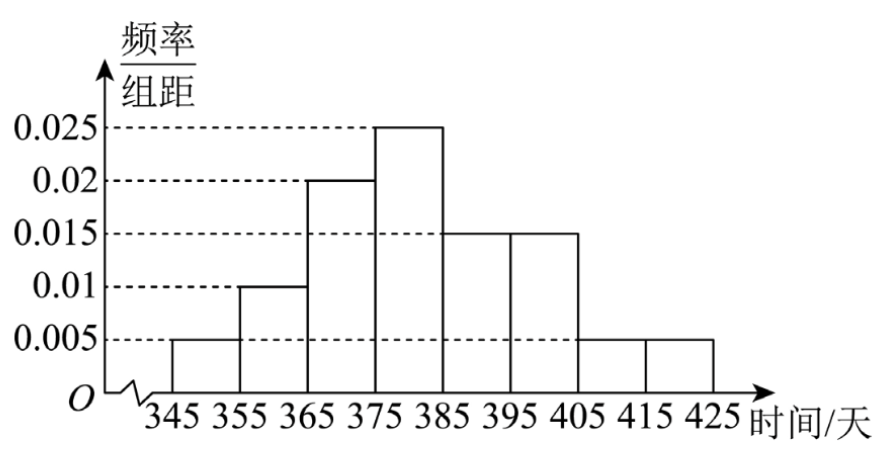
\includegraphics[width=0.62\linewidth]{figures/2026_xgk2_q15.png}
\end{tightcenter}

（1）求第一四分位数和中位数；

（2）$\hat p$ 为首次故障时间小于 $365$ 天的概率估计值.

（i）求 $\hat p$；

（ii）工厂向某用户销售 $100$ 件电子元件，$X$ 为这 $100$ 件产品首次出现故障小于 $365$ 天的件数，则 $X\sim B(100,\hat p)$，求 $E(X),D(X)$.

\item（15分）

三棱锥 $A-BCD$ 中，$E$ 在 $BD$ 上，$AE\perp CE,AE\perp DE,CD\perp AD$.

\noindent\begin{minipage}[t]{0.60\linewidth}
（1）证明：$CD\perp AB$；

（2）若 $DE=2,BE=1,AE=\sqrt2,CD=2\sqrt3$，求 $AD$ 与平面 $ABC$ 所成角的正弦值.
\end{minipage}\hfill
\begin{minipage}[t]{0.34\linewidth}
\vspace{-1.0em}
\centering
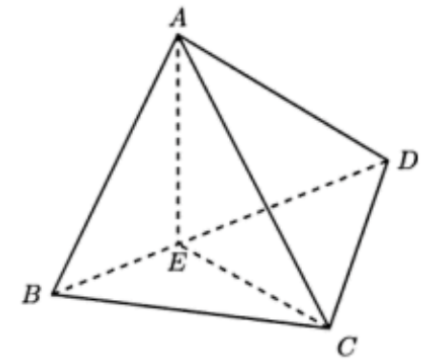
\includegraphics[width=\linewidth]{figures/2026_xgk2_q16.png}
\end{minipage}

\item（15分）

在 $\triangle ABC$ 中，已知 $\cos B=\dfrac34$，$\cos^2(A+C)+\sin A\sin C=1$.

（1）证明：$\triangle ABC$ 为钝角三角形；

（2）若 $\triangle ABC$ 面积为 $\dfrac{\sqrt7}{4}$，求 $\triangle ABC$ 周长.

\item（17分）

椭圆 $E:\dfrac{x^2}{a^2}+y^2=1(a>1)$，过右焦点垂直于 $x$ 轴的直线被 $E$ 所截线段长为 $\sqrt2$.

（1）求 $E$ 的离心率；

（2）$O$ 为坐标原点，给定点 $G(t_0,0)(t_0\neq0)$；$A(x_0,y_0)(y_0\neq0)$ 在 $E$ 上，过点 $A$ 作 $y$ 轴的垂线，交于点 $B$，$AO$ 与 $GB$ 交于点 $P$. 当 $A$ 在 $E$ 上运动时，$P$ 的轨迹为 $M$.

（i）求 $M$ 的方程；

（ii）$M$ 是否有中心点？当 $t_0$ 为何值时，$M$ 有中心点？当 $M$ 有中心点时，平移 $M$ 到 $M'$，使 $O$ 为 $M'$ 的中心点，说明 $M'$ 为何形状？

\item（17分）

已知函数 $f(x)=xe^x+ax+b$，曲线 $y=f(x)$ 在点 $(0,f(0))$ 处的切线方程为 $y=-2x+1$.

（1）求 $a,b$；

（2）当 $x>0$ 时，$f(x+m)-f(x)>m$，求 $m$ 的取值范围；

（3）当 $x>0$ 时，$f(x+k)+f(k-x)>2f(k)$，求 $k$ 的最小值.
\end{examanswers}

\end{document}